\documentclass[12pt]{article}

%% Comments

\usepackage{color}

\newif\ifcomments\commentstrue

\ifcomments
\newcommand{\authornote}[3]{\textcolor{#1}{[#3 ---#2]}}
\newcommand{\todo}[1]{\textcolor{red}{[TODO: #1]}}
\else
\newcommand{\authornote}[3]{}
\newcommand{\todo}[1]{}
\fi

\newcommand{\wss}[1]{\authornote{blue}{SS}{#1}} 
\newcommand{\plt}[1]{\authornote{magenta}{TPLT}{#1}} %For explanation of the template
\newcommand{\an}[1]{\authornote{cyan}{Author}{#1}}

%% Common Parts
\usepackage{booktabs}
\usepackage{tabularx}
\usepackage{hyperref}
\usepackage[round]{natbib}
\usepackage{amsmath, mathtools}
\usepackage{amsfonts}
\usepackage{amssymb}
\usepackage{graphicx}
\usepackage{colortbl}
\usepackage{xr}
\usepackage{longtable}
\usepackage{xfrac}
\usepackage{float}
\usepackage{siunitx}
\usepackage{caption}
\usepackage{pdflscape}
\usepackage{afterpage}
\usepackage{tikz}
\usetikzlibrary{mindmap}
\usepackage{multirow}
\usepackage{fullpage}
%\usepackage{refcheck}

\newcommand{\famname}{MIA}
\newcommand{\progname}{MISEG}

% For easy change of table widths
\newcommand{\colZwidth}{1.0\textwidth}
\newcommand{\colAwidth}{0.13\textwidth}
\newcommand{\colBwidth}{0.82\textwidth}
\newcommand{\colCwidth}{0.1\textwidth}
\newcommand{\colDwidth}{0.05\textwidth}
\newcommand{\colEwidth}{0.8\textwidth}
\newcommand{\colFwidth}{0.17\textwidth}
\newcommand{\colGwidth}{0.5\textwidth}
\newcommand{\colHwidth}{0.28\textwidth}

% Used so that cross-references have a meaningful prefix
\newcounter{defnum} %Definition Number
\newcommand{\dthedefnum}{GD\thedefnum}
\newcommand{\dref}[1]{GD\ref{#1}}
\newcounter{datadefnum} %Datadefinition Number
\newcommand{\ddthedatadefnum}{DD\thedatadefnum}
\newcommand{\ddref}[1]{DD\ref{#1}}
\newcounter{theorynum} %Theory Number
\newcommand{\tthetheorynum}{T\thetheorynum}
\newcommand{\tref}[1]{T\ref{#1}}
\newcounter{tablenum} %Table Number
\newcommand{\tbthetablenum}{T\thetablenum}
\newcommand{\tbref}[1]{TB\ref{#1}}
\newcounter{assumpnum} %Assumption Number
\newcommand{\atheassumpnum}{P\theassumpnum}
\newcommand{\aref}[1]{A\ref{#1}}
\newcounter{goalnum} %Goal Number
\newcommand{\gthegoalnum}{P\thegoalnum}
\newcommand{\gsref}[1]{GS\ref{#1}}
\newcounter{instnum} %Instance Number
\newcommand{\itheinstnum}{IM\theinstnum}
\newcommand{\iref}[1]{IM\ref{#1}}
\newcounter{reqnum} %Requirement Number
\newcommand{\rthereqnum}{P\thereqnum}
\newcommand{\rref}[1]{R\ref{#1}}
\newcounter{lcnum} %Likely change number
\newcommand{\lthelcnum}{LC\thelcnum}
\newcommand{\lcref}[1]{LC\ref{#1}}

\hypersetup{
    bookmarks=true,         % show bookmarks bar?
    colorlinks=true,       % false: boxed links; true: colored links
    linkcolor=red,          % color of internal links (change box color with linkbordercolor)
    citecolor=green,        % color of links to bibliography
    filecolor=magenta,      % color of file links
    urlcolor=cyan           % color of external links
}


%tikstyle commands
% Define block styles
\tikzstyle{context} = [rectangle, rounded corners, text width=2.5cm, minimum
size=2.5cm,text centered, draw=black, fill=white!30]
\tikzstyle{strategy} = [trapezium, trapezium left angle=70, trapezium right
angle=110, text width=3cm, minimum height=1cm, text centered, draw=black,
fill=white!30]
\tikzstyle{subclaim} = [rectangle, text width=3cm, minimum height=1cm, text
centered, draw=black, fill=white!30]
\tikzstyle{goal} = [rectangle, text width=5cm, minimum height=1cm, text
centered, draw=black, fill=white!30]
\tikzstyle{assumption} = [ellipse, text width=3cm, minimum height=1cm, text
centered, draw=black, fill=white!30]
\tikzstyle{evidence} = [circle, text width=2cm, minimum size=2cm, text
centered,draw=black, fill=white!30]
\tikzstyle{arrow} = [thick,->,>=stealth]

\begin{document}

\title{Software Requirements Specification for Medical Image Segmentation
Library}
\author{Ao Dong}
\date{\today}

\maketitle

~\newpage

\pagenumbering{roman}

\section{Revision History}

\begin{tabularx}{\textwidth}{p{3cm}p{2cm}X}
\toprule {\bf Date} & {\bf Version} & {\bf Notes}\\
\midrule
Oct 11 & 1.0 & Initial draft\\
Oct 15 & 1.1 & Revised according to GitHub issues\\
Oct 17 & 1.2 & Added more nonfunctional requirements\\
Oct 18 & 1.3 & Revised input image format and functional requirements\\
Oct 21 & 1.4 & Revised TM, IM and nonfunctional requirements\\
Dec 8 & 2.0 & Changed from CA to SRS\\
\bottomrule
\end{tabularx}

~\newpage
	
\section{Reference Material}

This section records information for easy reference.

\subsection{Table of Units}

Throughout this document SI (Syst\`{e}me International d'Unit\'{e}s) is
employed as the unit system. In addition to the basic units, several derived
units are
used as described below.  For each unit, the symbol is given followed by a
description of the unit and the SI name.
~\newline

\renewcommand{\arraystretch}{1.2}
%\begin{table}[ht]
  \noindent \begin{tabular}{l l l} 
    \toprule		
    \textbf{symbol} & \textbf{unit} & \textbf{SI}\\
    \midrule 
    N/A\\
    \bottomrule
  \end{tabular}
  %	\caption{Provide a caption}
%\end{table}

\subsection{Table of Symbols}

The table that follows summarizes the symbols used in this document along with
their units.  The choice of symbols was made to be consistent with the heat
transfer literature and with existing documentation for solar water heating
systems.  The symbols are listed in alphabetical order.

\renewcommand{\arraystretch}{1.2}
%\noindent \begin{tabularx}{1.0\textwidth}{l l X}
\noindent \begin{longtable*}{l l p{12cm}} \toprule
\textbf{symbol} & \textbf{unit} & \textbf{description}\\
\midrule 
$a$ & N/A & dimension of spatial coordinates
\\
$b$ & N/A & dimension of feature values
\\
$C_{1}$ & N/A & the first class with pixels in $[0, k]$
\\
$C_{2}$ & N/A & the second class with pixels in $[k+1, L-1]$
\\
$f$ & N/A & function defining an input image
\\
$F$ & N/A & input medical image
\\
$g$ & N/A & function defining an output image
\\
$G$ & N/A & output segmentation image
\\
$h$ & N/A & function defining a mathematical image
\\
$H$ & N/A & 2D digital grayscale image
\\
$i$ & N/A & intensity value
\\
$k$ & N/A & threshold value in Otsu' Method
\\
$k_{1}$ & N/A & threshold value in Otsu' Method with multiple thresholds
\\
$k_{2}$ & N/A & threshold value in Otsu' Method with multiple thresholds
\\
$k^{\star}$ & N/A & optimal  threshold  value found by Otsu' Method
\\
$k^{\star}_{1}$ & N/A & optimal threshold value found by Otsu' Method with
multiple thresholds
\\
$k^{\star}_{2}$ & N/A & optimal threshold value found by Otsu' Method with
multiple thresholds
\\
$L$ & N/A & number  of  the  discrete  levels  of  the  feature value
\\
$m_{1}$ & N/A & mean intensity of the pixels in $C_{1}$
\\
$m_{2}$ & N/A & mean intensity of the pixels in $C_{2}$
\\
$m_{3}$ & N/A & mean intensity of the pixels in the third class
\\
$m_{G}$ & N/A & mean global intensity
\\
$n_{i}$ & N/A & number of pixels of intensity $i$
\\
$\mathbb{N}$ & N/A & set of all natural numbers
\\
$p_{i}$ & N/A & normalized histogram
\\
$P_{1}$ & N/A & probability of the first class $C_{1}$
\\
$P_{2}$ & N/A & probability of the second class $C_{2}$
\\
$P_{3}$ & N/A & probability of the third class
\\
$\mathbb{R}$ & N/A & set of all real numbers
\\
$\sigma_{B}$ & N/A & between-class variance
\\
$T_{h}$ & N/A & threshold value for segmentation
\\
$x$ & N/A & x-axial coordinate of a image
\\
$y$ & N/A & y-axial coordinate of a image
\\
$X, X_i, X_o$ & N/A & x-axial pixel length of an (input or output) image
\\
$Y, Y_i, Y_o$ & N/A & y-axial pixel length of an (input or output) image
\\
$\mathbb{Z}$ & N/A & set of all integers
\\ 
\bottomrule
\end{longtable*}

\subsection{Abbreviations and Acronyms}

\renewcommand{\arraystretch}{1.2}
\begin{tabular}{l l} 
  \toprule		
  \textbf{symbol} & \textbf{description}\\
  \midrule 
  2D & Two-Dimensional\\
  3D & Three-Dimensional\\
  A & Assumption\\
  DD & Data Definition\\
  DICOM & Digital Imaging and Communications in Medicine\\
  GD & General Definition\\
  GS & Goal Statement\\
  IM & Instance Model\\
  LC & Likely Change\\
  MG & Module Guide\\
  \famname & Medical Image Applications\\
  MIS & Module Interface Specification\\
  \progname & Medical Image Segmentation Library\\
  PS & Physical System Description\\
  R & Requirement\\
  SRS & Software Requirements Specification\\
  T & Theoretical Model\\
  VTK & the Visualization Toolkit\\
  VnV & Verification and Validation\\
  \bottomrule
\end{tabular}\\

\newpage

\tableofcontents

~\newpage

\pagenumbering{arabic}

\section{Introduction}

Medical imaging technologies in medical diagnoses have become essential and
effective tools for professionals in medicine. Computers are also widely used
to generate, process, and visualize medical images. There is a big family of
computer software developed to serve these purposes.

The following sections provide an overview of the Software Requirements
Specification (SRS) for one software library - Medical Image Segmentation
Library (\progname) - in the family of Medical Imaging Applications (\famname).
This section explains the purpose of this document, the scope of the family,
the characteristics of the intended reader, and the organization of the document.
\subsection{Purpose of Document}

The major purpose of this document is to describe the specifications for
\progname and some commonalities of \famname. Goals, assumptions, theoretical
models, definitions, and other model derivation information are specified,
allowing the reader to fully understand and verify the purpose and scientific
basis of \famname. This SRS will remain abstract, describing what problem is
being solved, but not how to solve it.

This document will be used as a starting point for subsequent development
phases, including writing the design specification and the software
verification and validation plan. The design document will show how the
requirements are to
be realized, including decisions
on the numerical algorithms and programming environment. The verification and
validation plan will show the steps that will be used to increase confidence in
the software documentation and the implementation. Although the SRS fits in a
series of documents that follow the so-called waterfall model, the actual
development process is not constrained in any way. Even when the waterfall
model is not followed, as \cite{ParnasAndClements1986} point out, the most
logical wayto present the documentation is still to “fake” a rational design
process.

\subsection{Scope of the Family and the Software} 

According to \cite{Bankman2000}, \famname{} deal with 6 different basic
problems, while \cite{Angenent2006} pointed out that 4 fundamental problems are
solved by \famname. While both mentioned Segmentation, Registration and
Visualization of medical images, Bankman also included Enhancement,
Quantification and a section covering some other functions~\cite{Bankman2000}.
On the other hand, Angenent's team included Simulation~\cite{Angenent2006}.
According to \cite{wiki:001}, \famname{} have major functions in categories
suchas Segmentation, Registration, Visualization (including the basic display,
reformatted views and 3D volume rendering), Statistical Analysis, Image-based
Physiological Modelling, etc. As \cite{Kim2011} describe, the general steps of
medical image analysis after obtaining digital data include Enhancement,
Segmentation, Feature Extraction, Classification and Interpretation.

The major functions of \famname{} can be divided into several sections and sub
sections as shown in Figure \ref{fg_miafunctions}.

\begin{center}
\begin{tikzpicture}[mindmap, grow cyclic, every node/.style=concept, concept
color=orange!40,
	level 1/.append style={level distance=5cm,sibling angle=90},
	level 2/.append style={level distance=3cm,sibling angle=90},
	level 3/.style={level distance=3cm,sibling angle=60}]
\node{\famname}
	child[concept color=teal!40] { node {Enhancement}}
	child[concept color=teal!40] { node {Analysis}
    	child[concept color=blue!30] { node {Registration}}
	    child[concept color=purple!50,] { node {Segmentation}}
	    child[concept color=blue!30] { node {Statistical Analysis}
	        child { node {Feature Extraction}}
	        child { node {Classification}}
	        child { node {Interpretation}}
	}}
	child[concept color=teal!40] { node {Simulation/\\Modeling}}
    child[concept color=teal!40] { node {Visualization}
	    child[concept color=blue!30] { node {2D Display}}
	    child[concept color=blue!30] { node {3D Rendering}}
	    child[concept color=blue!30] { node {Reformatted Views}}
    	}
;
\end{tikzpicture}
\captionof{figure}{Major functions of \famname}
\label{fg_miafunctions}
\end{center}

In this project, the scope of the software is limited to the software library
providing the segmentation tools and functions.

\subsection{Characteristics of Intended Reader} 

Reviewers of this documentation should have an understanding of functions, sets
and binary numbers in discrete math from level 1 or 2 computer science and
probability from level 1 and 2 calculus.

The users of \progname{} can have a lower level of expertise, as explained in
Section \ref{sec_UserCharacteristics}.


\subsection{Organization of Document}

The organization of this document follows the template for an SRS for
scientific computing software proposed by \cite{Parnas1972} and
\cite{ParnasAndClements1986}. The presentation follows the standard pattern of
presenting goals, theories, definitions, and assumptions. For readers that
would like a more bottom up approach, they can start reading the instance
models in Section \ref{sec_instance} and trace back to find any additional
information they require.
The goal statements (Section \ref{sec_goalstatements}) are refined to the
theoretical models and the theoretical models (Section \ref{sec_theoretical})
to the instance models (Section \ref{sec_instance}). The instance models to be
solved are referred to as \iref{IM_singlethres}, \iref{IM_singlethresoutput},
\iref{IM_multithres}, \iref{IM_multithresoutput}.

\section{General System Description}

This section identifies the interfaces between the system and its environment,
describes the potential user characteristics and lists the potential system
constraints.

\subsection{Potential System Contexts}

Figure \ref{fg_syscontext} shows the system context. A circle represents an
external entity outside the software, the user in this case. A rectangle
represents the software system itself (\famname).
Arrows are used to show the data flow between the system and its environment.
\progname{} are mostly self-contained. The only external interaction is through
the user interface. The responsibilities of the user and the system are as
follows:

\begin{itemize}
\item User Responsibilities:
\begin{itemize}
\item Provide the input data to the system
\item Given two or more options by the system, decide to use which calculation
method
\end{itemize}
\item \progname{} Responsibilities:
\begin{itemize}
\item Detect data type mismatch, such as a text file instead of a image file
\item Determine if the inputs satisfy the required mathematical and software
constraints
\item Calculate the required outputs
\end{itemize}
\end{itemize}

\begin{center}
\begin{tikzpicture}
    \node (n1) [evidence] {User};
    \node (n2) [context ,right of= n1, node distance = 2.1in] {\famname};
    \node (n3) [evidence, right of= n2, node distance = 4.4in] {User};
    \draw [arrow] (n1.0)  -- node[above]{Medical Image}  (n2.180);
\draw [arrow] (n2.0) -- node[above]{Optimal threshold values, segmentation
image} (n3.180);
\end{tikzpicture}
\captionof{figure}{System Context}
\label{fg_syscontext}
\end{center}

\subsection{Potential User Characteristics} \label{sec_UserCharacteristics}

The end user of \progname{} should have an understanding of undergraduate Level
1 Calculus and Physics.

\subsection{Potential System Constraints}

There are no system constraints.

\section{Specific System Description}
This section first presents the problem description, which gives a high-level
view of the
problem to be solved. This is followed by the solution characteristics
specification, which
presents the assumptions, theories, definitions and finally the instance
models.\subsection{Problem Description} \label{sec_ProblemDes}
Segmentation, separation of structures of interest from the background and from
each other~\cite{Bankman2000}. Image segmentation is the process of
partitioning an image into different meaningful segments. In medical imaging,
these segments
often correspond to different tissue classes, organs, pathologies, or other
biologically relevant structures~\cite{Forouzanfar2010}. Image segmentation is
one of the most interesting and challenging problems in computer vision
generally and medical imaging applications specifically~\cite{Elnakib2011}.

Regarding the different medical image segmentation methods, \cite{Withey2007}
suggested that they can be divided into 3 generations from low-level to
high-level technologies as shown in table \ref{fg_segmethods}.

This document is focusing on the Intensity Threshold method.

\begin{center}
\begin{table}[h]
\begin{tabular}{|c|l|l|l|}
\hline
\multirow{2}{*}{\textbf{Generation}} & \multicolumn{3}{c|}{\textbf{Category}}
\\\cline{2-4}
& \multicolumn{1}{c|}{\textbf{Region-based}} &
\multicolumn{1}{c|}{\textbf{\begin{tabular}[c]{@{}c@{}}Boundary\\
Following\end{tabular}}} &
\multicolumn{1}{c|}{\textbf{\begin{tabular}[c]{@{}c@{}}Pixel\\
Classification\end{tabular}}} \\ \hline
\textbf{$1^{st}$} & • Region growing & \begin{tabular}[c]{@{}l@{}}• Edge
tracing\\ (heuristic)\end{tabular} & • Intensity threshold \\ \hline
\textbf{$2^{nd}$} & \begin{tabular}[c]{@{}l@{}}• Deformable models\\ • Graph
search\end{tabular} & \begin{tabular}[c]{@{}l@{}}• Minimal path\\ • Target
tracking\\ • Graph search\\ • Neural networks\\ • Multi resolution\end{tabular}
&\begin{tabular}[c]{@{}l@{}}• Statistical pattern recognition\\ • C-means
clustering\\ • Neural networks\\ • Multi resolution\end{tabular} \\ \hline
\textbf{$3^{rd}$} & \begin{tabular}[c]{@{}l@{}}• Shape models\\ • Appearance
models\\ • Rule-based\\ • Coupled surfaces\end{tabular} & &
\begin{tabular}[c]{@{}l@{}}• Atlas-based\\ • Rule-based\end{tabular} \\ \hline
\end{tabular}
\caption{Segmentation Methods~\cite{Withey2007}}
\label{fg_segmethods}
\end{table}
\end{center}

\subsubsection{Terminology and  Definitions}

This subsection provides a list of terms that are used in the subsequent
sections and their meaning, with the purpose of reducing ambiguity and making
it easier to correctly understand the requirements:

\begin{itemize}

\item Image: in Mathematics, an image is defined as a function
  $h : \mathbb{R}^{a} \rightarrow \mathbb{R}^{b}$.
\item Digital image: When the spatial coordinates and the function value are
  finite and discrete, the image is called digital, shown as
  $h : \mathbb{Z}^{a} \rightarrow \mathbb{Z}^{b}$.
\item Grayscale image: In digital photography, computer-generated imagery, and
  colorimetry, a grayscale or grayscale image is one in which the value of each
  pixel is a single sample representing only an amount of light, that is, it
  carries only intensity information.
\item 2D Digital Image: the computer-based generation of digital images -
mostly from two-dimensional models (such as 2D geometric models, text, and
digital
  images) and by techniques specific to them.
\item Medical Image: visual representations of the interior of a body for
  clinical analysis and medical intervention, as well as visual representation
  of the function of some organs or tissues (physiology).
\item Grayscale Intensity: represents gray levels, where the intensity 0
usually represents black and the intensity 255 usually represents full
intensity,or
  white.
\item Shades of Gray: variations of gray or grey include achromatic grayscale
  shades, which lie exactly between white and black, and nearby colors with low
  colorfulness.
\item Coordinates: in geometry, a coordinate system is a system that uses one
or more numbers, or coordinates, to uniquely determine the position of the
points or other geometric elements on a manifold such as Euclidean space.
\item Histogram: a histogram is an accurate representation of the distribution
  of numerical data. It is an estimate of the probability distribution of a
  continuous variable.
\item Pixel: in digital imaging, a pixel, pel, or picture element is a physical
  point in a raster image, or the smallest addressable element in an all points
  addressable display device; so it is the smallest controllable element of a
  picture represented on the screen.
\item VTK: the Visualization Toolkit is an open-source, freely available
  software system for 3D computer graphics, modeling, image processing, volume
  rendering, scientific visualization, and 2D plotting.
\item DICOM: Digital Imaging and Communications in Medicine (DICOM) is the
  standard for the communication and management of medical imaging information
  and related data.
\end{itemize}

\subsubsection{Goal Statements}
\label{sec_goalstatements}
\noindent Given the medical images as inputs, the goal statements are:

\begin{itemize}

\item[GS\refstepcounter{goalnum}\thegoalnum \label{GS_calk}:]
Calculate and display the optimal threshold value $k^{\star}$ with Otsu’s
Method.

\item[GS\refstepcounter{goalnum}\thegoalnum \label{GS_outputimage}:]
Output the processed images representing the segmentation results with one
threshold.

\item[GS\refstepcounter{goalnum}\thegoalnum \label{GS_multicalk}:]
Calculate and display multiple optimal threshold values $k^{\star}_{1}$ and
$k^{\star}_{2}$ with Otsu’s Method.

\item[GS\refstepcounter{goalnum}\thegoalnum \label{GS_multioutputimage}:]
Output the processed images representing the segmentation results with multiple
thresholds.

\end{itemize}

\subsection{Solution Characteristics Specification}

\begin{figure}[H]
  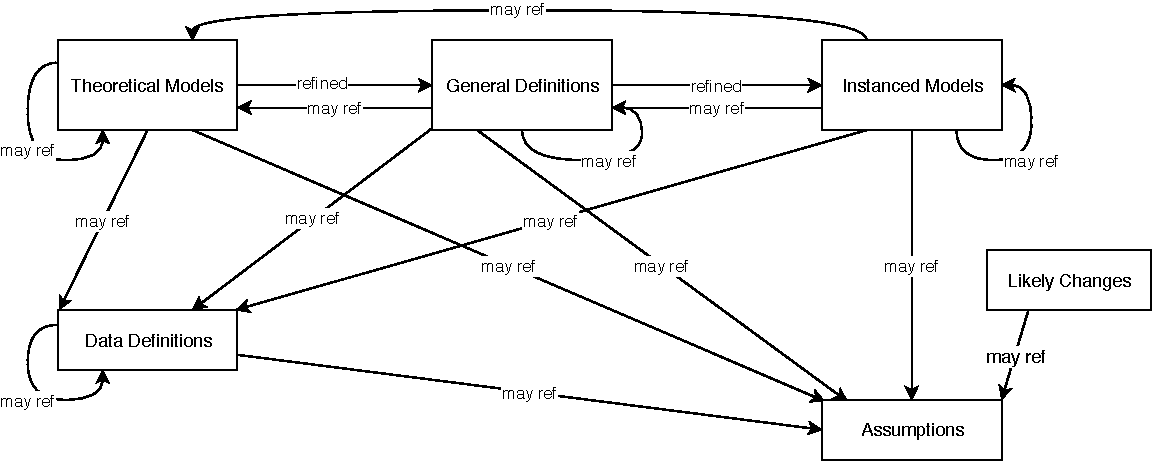
\includegraphics[scale=0.9]{RelationsBetweenTM_GD_IM_DD_A.pdf}
\end{figure}

The instance models that govern \progname{} are presented in
Subsection~\ref{sec_instance}. The information to understand the meaning of
the instance models and their derivation is also presented, so that the instance
models can be verified.

\subsubsection{Assumptions}
\label{sec_assumpt}

\begin{itemize}

\item[A\refstepcounter{assumpnum}\theassumpnum \label{A_2Dgrayscale}:]
The images are 2D and grayscale.

\item[A\refstepcounter{assumpnum}\theassumpnum \label{A_8bitinteger}:]
The pixel format of input images is DICOM image, where the feature value is the
gray intensity value stored as an 12-bit or 16-bit integer giving a range of
possible values from 0 to 4095 or 65535.

The pixel format of output images is the byte image, where the feature value is
the gray intensity value stored as an 8-bit integer giving a range of possible
values from 0 to 255.

\end{itemize}

\subsubsection{Theoretical Models} \label{sec_theoretical}

This section focuses on the general equations and laws that \progname{} is
based on.

~\newline

\noindent
\begin{minipage}{\textwidth}
\renewcommand*{\arraystretch}{1.5}
\begin{tabular}{| p{\colAwidth} | p{\colBwidth}|}
  \hline
  \rowcolor[gray]{0.9}
  Number& T\refstepcounter{theorynum}\thetheorynum \label{T_mathimage}\\
  \hline
  Label&\bf Mathematical Image\\
  \hline
  Equation&  $h : \mathbb{R}^{a} \rightarrow \mathbb{R}^{b}$\\
  \hline
  Description & 
In Mathematics, an image is defined as a function $h : \mathbb{R}^{a}
\rightarrow \mathbb{R}^{b}$, where $\mathbb{R}^{a}$ denotes the set of
a-dimensional spatial coordinates and $\mathbb{R}^{b}$ the set of b-dimensional
feature values.\\
  \hline
  Source &  \cite{Ferrari2018a}\\
% The above web link should be replaced with a proper citation to a publication
\hline
  Ref.\ By & \ddref{DD_digitalimage}\\
  \hline
\end{tabular}
\end{minipage}\\

~\newline

\noindent
\begin{minipage}{\textwidth}
\renewcommand*{\arraystretch}{1.5}
\begin{tabular}{| p{\colAwidth} | p{\colBwidth}|}
  \hline
  \rowcolor[gray]{0.9}
  Number& T\refstepcounter{theorynum}\thetheorynum \label{T_singlethres}\\
  \hline
  Label&\bf Single Global Threshold Method\\
  \hline
  Equation&  $g(x,y)=\left\{
\begin{aligned}
&L-1,\ &if\ f(x,y)>T_{h} \\
&0,\ &if\ f(x,y)\leq T_{h}
\end{aligned}
\right.$\\
  \hline
  Description & 
$f(x,y)$ and $g(x,y)$ are the feature values at $(x,y)$ of the input and output
image respectively. $L$ is the number of the discrete levels of the feature
value. $T_{h}$ is the threshold value.\\
  \hline
  Source &  \cite{Ferrari2018b}\\
% The above web link should be replaced with a proper citation to a publication
\hline
Ref.\ By & \ddref{DD_betweenvariance} \tref{T_multithres}
\iref{IM_singlethresoutput}\\
  \hline
\end{tabular}
\end{minipage}\\

~\newline

\noindent
\begin{minipage}{\textwidth}
\renewcommand*{\arraystretch}{1.5}
\begin{tabular}{| p{\colAwidth} | p{\colBwidth}|}
  \hline
  \rowcolor[gray]{0.9}
  Number& T\refstepcounter{theorynum}\thetheorynum \label{T_multithres}\\
  \hline
  Label&\bf Multiple Global Thresholds Method\\
  \hline
  Equation&  $g(x,y)=\left\{
\begin{aligned}
&L-1,\ &if\ f(x,y) > T_{h2} \\
&L/2,\ &if\ T_{h1} < f(x,y) \leq T_{h2}\\
&0,\ &if\ f(x,y) \leq T_{h1}
\end{aligned}
\right.$\\
  \hline
  Description & 
$f(x,y)$ and $g(x,y)$ are the feature values at $(x,y)$ of the input and output
image respectively. $L$ is the number of the discrete levels of the feature
value. $T_{h1}$ and $T_{h2}$ are the threshold values.\\
  \hline
  Source &  \cite{Ferrari2018b}\\
% The above web link should be replaced with a proper citation to a publication
\hline
  Ref.\ By & \iref{IM_multithresoutput}\\
  \hline
\end{tabular}
\end{minipage}\\

~\newline

\noindent
\begin{minipage}{\textwidth}
\renewcommand*{\arraystretch}{1.5}
\begin{tabular}{| p{\colAwidth} | p{\colBwidth}|}
  \hline
  \rowcolor[gray]{0.9}
  Number& T\refstepcounter{theorynum}\thetheorynum \label{T_otsu}\\
  \hline
  Label&\bf Otsu's Method\\
  \hline
Equation& $\sigma^{2}_{B}(k^{\star}) =
\underset{0<k<L-1}{max}\sigma^{2}_{B}(k)$\\
  \hline
  Description & 
Otsu’s method is aimed in finding the optimal value for the global threshold
$T$. The optimal threshold value, $k^{\star}$, satisfies the above equation,
where using $k$ as threshold to divide all pixels of the image into two
classes:$C_{1}$ (pixels in $[0, k]$) and $C_{2}$ (pixels in $[k + 1, L - 1]$).
$\sigma_{B}$ is the between-class variance.\\
  \hline
  Source &  \cite{Ferrari2018b}\\
% The above web link should be replaced with a proper citation to a publication
\hline
  Ref.\ By & \iref{IM_singlethres} \iref{IM_multithres}\\
  \hline
\end{tabular}
\end{minipage}\\

~\newline

\subsubsection{Data Definitions} \label{sec_datadef}

This section collects and defines all the data needed to build the instance
models. The dimension of each quantity is also given.

~\newline

\noindent
\begin{minipage}{\textwidth}
\renewcommand*{\arraystretch}{1.5}
\begin{tabular}{| p{\colAwidth} | p{\colBwidth}|}
\hline
\rowcolor[gray]{0.9}
Number& DD\refstepcounter{datadefnum}\thedatadefnum \label{DD_digitalimage}\\
\hline
Label& \bf Digital Image\\
\hline
Symbol & N/A\\
\hline
% Units& $Mt^{-3}$\\
% \hline
  SI Units & N/A\\
  \hline
  Equation & $h : \mathbb{Z}^{a} \rightarrow \mathbb{Z}^{b}$\\
  \hline
  Description & 
    In Mathematics, an image is defined as a function $h : \mathbb{R}^{a}
                \rightarrow \mathbb{R}^{b}$. Usually, $a = 2$ and, in the
                simplest case, $b = 1$. When the spatial coordinates and the
                function value are finite and discrete, the image is called
                digital, shown as $h : \mathbb{Z}^{a} \rightarrow
                \mathbb{Z}^{b}$.
  \\
  \hline
  Sources& \cite{Ferrari2018a}\\
  \hline
  Ref.\ By & \ddref{DD_2DGrayscale}\\
  \hline
\end{tabular}
\end{minipage}\\

~\newline

\noindent
\begin{minipage}{\textwidth}
\renewcommand*{\arraystretch}{1.5}
\begin{tabular}{| p{\colAwidth} | p{\colBwidth}|}
\hline
\rowcolor[gray]{0.9}
Number& DD\refstepcounter{datadefnum}\thedatadefnum \label{DD_2DGrayscale}\\
\hline
Label& \bf 2D Digital Grayscale Image\\
\hline
Symbol & $H$\\
\hline
% Units& $Mt^{-3}$\\
% \hline
  SI Units & N/A\\
  \hline
Equation & $H_{X \times Y} = [h(x,y)]_{X \times Y}$ where $h(x,y) \in
\{0,1,...,L-1\}$\\
  \hline
  Description & 
In this project, we only consider 2D grayscale images, as stated in
\aref{A_2Dgrayscale}. The images can be defined as $h : \mathbb{Z}^{2}
\rightarrow \mathbb{Z}$, or the above equation. $X \times Y$ is the size of the
image. $(x,y)$ denotes the 2D spatial coordinates, where $x \in [0,X-1]$ and $y
\in [0,Y-1]$. $h(x,y)$ denotes the
feature values at $(x,y)$ of the image. Depending on the type of image, the
feature value
                could be light intensity, depth, intensity of radio wave or
                temperature. $\{0,1,...,L-1\}$ is the set of discrete levels of
                the feature value, and $L$ is the number of the levels. In this
                project, we refer to $h(x,y)$ as gray intensity
                value (or intensity) at $(x,y)$.
  \\
  \hline
  Sources& \cite{Pal1993}\\
  \hline
Ref.\ By & \ddref{DD_betweenvariance} \tref{T_singlethres} \tref{T_multithres}
\iref{IM_singlethres}\iref{IM_multithres}\\
  \hline
\end{tabular}
\end{minipage}\\

\wss{I also don't think this is adding anything new. If the new thing is the
output type, then couldn't you work that into your previous definitions?}
\an{I combined it into the above DD}

\wss{I'm not sure what this DD says that the previosu one doesn't already say.
In other DDs you will define the output, but this one doesn't really define the
output, it just says that there will be output.}
\an{I deleted that DD}

~\newline

\noindent
\begin{minipage}{\textwidth}
\renewcommand*{\arraystretch}{1.5}
\begin{tabular}{| p{\colAwidth} | p{\colBwidth}|}
\hline
\rowcolor[gray]{0.9}
Number& DD\refstepcounter{datadefnum}\thedatadefnum
\label{DD_pixelvalue}\\
\hline
Label& \bf Number of the shades of gray\\
\hline
Symbol & $L$\\
\hline
% Units& $Mt^{-3}$\\
% \hline
  SI Units & N/A\\
  \hline
  Equation & $L \in \{2^n | n \in \mathbb{N}\}$\\
  \hline
    Description & 
    $L$ is the number of the shades of gray, also referred as number of
intensity levels, where $n \in \{8, 12, 16 \}$, as stated in
\aref{A_8bitinteger}.
  \\
  \hline
  Sources& \url{https://homepages.inf.ed.ac.uk/rbf/HIPR2/value.htm}\\
  \hline
Ref.\ By & \ddref{DD_thresvalue} \ddref{DD_betweenvariance}
\tref{T_singlethres}\tref{T_multithres} \tref{T_otsu}
\iref{IM_singlethres}\iref{IM_multithres}\\
  \hline
\end{tabular}
\end{minipage}\\

~\newline

\noindent
\begin{minipage}{\textwidth}
\renewcommand*{\arraystretch}{1.5}
\begin{tabular}{| p{\colAwidth} | p{\colBwidth}|}
\hline
\rowcolor[gray]{0.9}
Number& DD\refstepcounter{datadefnum}\thedatadefnum \label{DD_thresvalue}\\
\hline
Label& \bf Threshold Value\\
\hline
Symbol & $T_{h}$\\
\hline
% Units& $Mt^{-3}$\\
% \hline
  SI Units & N/A\\
  \hline
  Equation & $T_{h} \in \{1,...,L-2\}$\\
  \hline
  Description & 
In this project, we refer to $h(x,y)$ gray intensity value (or intensity) at
$(x,y)$. Then, $T_{h} \in [1,254]$.
  \\
  \hline
  Sources& \cite{Ferrari2018b}\\
  \hline
Ref.\ By & \ddref{DD_betweenvariance} \tref{T_singlethres} \tref{T_multithres}
\iref{IM_singlethres}\iref{IM_multithres}\\
  \hline
\end{tabular}
\end{minipage}\\

~\newline

\noindent
\begin{minipage}{\textwidth}
\renewcommand*{\arraystretch}{1.5}
\begin{tabular}{| p{\colAwidth} | p{\colBwidth}|}
\hline
\rowcolor[gray]{0.9}
Number& DD\refstepcounter{datadefnum}\thedatadefnum
\label{DD_betweenvariance}\\\hline
Label& \bf Between-class Variance\\
\hline
Symbol & $\sigma^{2}_{B}$\\
\hline
% Units& $Mt^{-3}$\\
% \hline
  SI Units & N/A\\
  \hline
Equation & $\sigma^{2}_{B} = P_{1}(m_{1} - m_{G})^{2} + P_{2}(m_{2} -
m_{G})^{2}$\\
  \hline
  Description &
$n_{i}$ is the number of pixels of intensity $i$, where $i \in
\{0,1,...,L-1\}.$$p_{i}$ is the normalized histogram, where
    
    $p_{i} = \frac{n_{i}}{\sum_{i=1}^{L-1} n_{i}}$.
    
Using $k, 0 < k < L - 1$, as threshold, there are two classes: $C_{1}$ (pixels
in $[0, k]$) and $C_{2}$ (pixels in $[k + 1, L - 1]$).

    $P_{1}$ is the probability of the class $C_{1}$, where 
    
    $P_{1} = P(C_{1}) = \sum_{i=1}^{k} p_{i}$.
    
    $P_{2}$ is the probability of the class $C_{2}$, where 
    
    $P_{2} = P(C_{2}) = \sum_{i=k+1}^{L-1} p_{i} = 1 - P_{1}$.
    
    $m_{1}$ is the mean intensity of the pixels in $C_{1}$, where
    
$m_{1} = \sum_{i=1}^{k} i \cdot P(i | C_{1}) = \sum_{i=1}^{k} i \cdot
\frac{P(C_{1}|i)P(i)}{P(C_{1})} = \frac{1}{P_{1}}\sum_{i=1}^{k} i \cdot p_{i}$,
since $P(C_{1}|i)=1, P(i)=p_{i}$, and $P(C_{1})=P_{1}$.
    
    $m_{2}$ is the mean intensity of the pixels in $C_{2}$, similarly
    
    $m_{2} = \frac{1}{P_{2}}\sum_{i=k}^{L-1} i \cdot p_{i}$.
    
    $m_{G}$ is the mean global intensity, where
    
    $m_{G} = \sum_{i=1}^{L-1} i \cdot p_{i}$.
  \\
  \hline
  Sources& \cite{Ferrari2018b}\\
  \hline
  Ref.\ By & \tref{T_otsu} \iref{IM_singlethres} \iref{IM_multithres}\\
  \hline
\end{tabular}
\end{minipage}\\

~\newline

\subsubsection{Instance Models} \label{sec_instance}    

This section transforms the problem defined in Section~\ref{sec_ProblemDes}
into one which is expressed in mathematical terms. It uses concrete symbols
defined
in Section~\ref{sec_datadef} to replace the abstract symbols in the models
identified in Sections~\ref{sec_theoretical}.

Medical image segmentation by Threshold Method can be solved by
\tref{T_singlethres}, \tref{T_otsu}, \ddref{DD_2DGrayscale},
\ddref{DD_pixelvalue},
\ddref{DD_thresvalue}

~\newline

\noindent
\begin{minipage}{\textwidth}
\renewcommand*{\arraystretch}{1.5}
\begin{tabular}{| p{\colAwidth} | p{\colBwidth}|}
  \hline
  \rowcolor[gray]{0.9}
  Number& IM\refstepcounter{instnum}\theinstnum \label{IM_singlethres}\\
  \hline
Label& \bf Otsu's Method to find the single optimal threshold value
$k^{\star}$\\
  \hline
Input& $H_{X \times Y}, h(x,y)$ from \ddref{DD_2DGrayscale}, $L$ from
\ddref{DD_pixelvalue}, $\sigma_{B}$, k, $P_{1}$, $P_{2}$, $m_{1}$,
$m_{2}$, $m_{G}$ from \ddref{DD_betweenvariance}\\
  \hline
  Output& $k^{\star}$, such that\\
  & $\sigma^{2}_{B}(k^{\star}) = \underset{0<k<L-1}{max}\sigma^{2}_{B}(k)$\\
  \hline
  Description&
        Since $P_{1}m_{1} + P_{2}m_{2} = m_{G}$ and $P_{1} + P_{2} = 1$,
        
$\sigma^{2}_{B} = P_{1}(m_{1} - m_{G})^{2} + P_{2}(m_{2} - m_{G})^{2} =
P_{1}P_{2}(m_{1} - m_{2})^{2}$
        
        Hence, for each value of $k$, $\sigma_{B}$ can be computed, where 
        
        $\sigma^{2}_{B}(k) = P_{1}(k)P_{2}(k)(m_{1}(k) - m_{2}(k))^{2}$
  \\
  \hline
  Sources& \cite{Ferrari2018b} \\
  \hline
  Ref.\ By & \iref{IM_singlethresoutput}\\
  \hline
\end{tabular}
\end{minipage}\\

~\newline

\noindent
\begin{minipage}{\textwidth}
\renewcommand*{\arraystretch}{1.5}
\begin{tabular}{| p{\colAwidth} | p{\colBwidth}|}
  \hline
  \rowcolor[gray]{0.9}
  Number& IM\refstepcounter{instnum}\theinstnum \label{IM_singlethresoutput}\\
  \hline
  Label& \bf Use single global threshold to output segmentation image\\
  \hline
Input& $H_{X \times Y}, h(x,y)$ from \ddref{DD_2DGrayscale}, $L$ from
\ddref{DD_pixelvalue}, $k^{\star}$ from \iref{IM_singlethres}\\
  \hline
  Output& $G_{X \times Y}$, such that for pixel at each $(x,y)$,
  
  $g(x,y)=\left\{
\begin{aligned}
&255,\ &if\ f(x,y)>k^{\star} \\
&0,\ &if\ f(x,y)\leq k^{\star}
\end{aligned}
\right.$\\
  \hline
  Description&
The output image $G_{X \times Y}$ has the same size and format as the input
image $F_{X \times Y}$. As a piece of 8-bit grayscale image, all of its pixels
are with intensity of either 255 or 0, so it only shows the same information as
a binary image.
  \\
  \hline
  Sources& \cite{Ferrari2018b} \\
  \hline
  Ref.\ By &\\
  \hline
\end{tabular}
\end{minipage}\\

~\newline

\noindent
\begin{minipage}{\textwidth}
\renewcommand*{\arraystretch}{1.5}
\begin{tabular}{| p{\colAwidth} | p{\colBwidth}|}
  \hline
  \rowcolor[gray]{0.9}
  Number& IM\refstepcounter{instnum}\theinstnum \label{IM_multithres}\\
  \hline
Label& \bf Otsu's Method to find the multiple optimal threshold values
$k^{\star}_{1}$ and $k^{\star}_{2}$\\
  \hline
Input& $H_{X \times Y}, h(x,y)$ from \ddref{DD_2DGrayscale}, $L$ from
\ddref{DD_pixelvalue}, $\sigma_{B}$, k, $P_{1}$, $P_{2}$, $m_{1}$,
$m_{2}$, $m_{G}$ from \ddref{DD_betweenvariance}\\
  \hline
  Output& $k^{\star}_{1}$ and $k^{\star}_{2}$, such that\\
& $\sigma^{2}_{B}(k^{\star}_{1}, k^{\star}_{2}) =
\underset{0<k_{1}<k_{2}<L-1}{max}\sigma^{2}_{B}(k_{1}, k_{2})$\\
  \hline
  Description&
        Similarly as the normal Otsu's Method,
        
$\sigma^{2}_{B}(k_{1}, k_{2}) = P_{1}(k_{1})(m_{1}(k_{1}) - m_{G})^{2} +
P_{2}(k_{2})(m_{2}(k_{2}) - m_{G})^{2} + P_{3}(k_{3})(m_{3}(k_{3}) -
m_{G})^{2}$\\
  \hline
  Sources& \cite{Ferrari2018b} \\
  \hline
  Ref.\ By & \iref{IM_multithresoutput}\\
  \hline
\end{tabular}
\end{minipage}\\

~\newline

\noindent
\begin{minipage}{\textwidth}
\renewcommand*{\arraystretch}{1.5}
\begin{tabular}{| p{\colAwidth} | p{\colBwidth}|}
  \hline
  \rowcolor[gray]{0.9}
  Number& IM\refstepcounter{instnum}\theinstnum \label{IM_multithresoutput}\\
  \hline
  Label& \bf Use multiple global thresholds to output segmentation image\\
  \hline
Input& $H_{X \times Y}, h(x,y)$ from \ddref{DD_2DGrayscale}, $L$ from
\ddref{DD_pixelvalue}, $k^{\star}_{1}$ and $k^{\star}_{2}$ from
\iref{IM_multithres}\\
  \hline
  Output& $G_{X \times Y}$, such that for pixel at each $(x,y)$,
  
  $g(x,y)=\left\{
\begin{aligned}
&255,\ &if\ f(x,y) > k^{\star}_{2} \\
&128,\ &if\ k^{\star}_{1} < f(x,y) \leq k^{\star}_{2}\\
&0,\ &if\ f(x,y) \leq k^{\star}_{1}
\end{aligned}
\right.$\\
  \hline
  Description&
The output image $G_{X \times Y}$ has the same size and format as the input
image $F_{X \times Y}$. As a piece of 8-bit grayscale image, all of its pixels
are with intensity of 255, 188 or 0, so it shows more information than a binary
image.
  \\
  \hline
  Sources& \cite{Ferrari2018b} \\
  \hline
  Ref.\ By &\\
  \hline
\end{tabular}
\end{minipage}\\

\subsubsection{Input Data Constraints} \label{sec_DataConstraints}    

Table~\ref{TblInputVar} shows the data constraints on the input output
variables.  The column for physical constraints gives the physical limitations
on the range of values that can be taken by the variable.  The column for
software constraints restricts the range of inputs to reasonable values.  The
software constraints will be helpful in the design stage for picking suitable
algorithms. The constraints are conservative, to give the user of the model
the flexibility to experiment with unusual situations. The column of typical
values is intended to provide a feel for a common scenario. The uncertainty
column
provides an estimate of the confidence with which the physical quantities can
be measured. This information would be part of the input if one were performing
an uncertainty quantification exercise.

\begin{table}[!h]
  \caption{Input Variables} \label{TblInputVar}
  \renewcommand{\arraystretch}{1.2}
\noindent \begin{longtable*}{l l l l c} 
  \toprule
\textbf{Var} & \textbf{Physical Constraints} & \textbf{Software Constraints} &
\textbf{Typical Value} & \textbf{Uncertainty}\\
  \midrule 
  $X_i$ & $X_i > 0$ & & 512 & 
  \\
  $Y_i$ & $Y_i > 0$ & & 512 & 
  \\
  $f(x,y)$ & $f(x,y) \ge 0$ & $PV_{MIN} \le f(x,y) \le PV_{MAX}$ & 128 & 
  \\
  \bottomrule
\end{longtable*}
\end{table}

\begin{table}[!h]
\caption{Specification Parameter Values} \label{TblSpecParams}
\renewcommand{\arraystretch}{1.2}
\noindent \begin{longtable*}{l l} 
  \toprule
  \textbf{Var} & \textbf{Value} \\
  \midrule 
  $PV_{MIN}$ & 0\\
  $PV_{MAX}$ & 255\\
  \bottomrule
\end{longtable*}
\end{table}

\subsubsection{Properties of a Correct Solution} \label{sec_CorrectSolution}

\noindent
A correct solution must exhibit valid optimal thresholds and a output image
with the same resolution as the input one and with valid pixel values.

\begin{table}[!h]
\caption{Output Variables} \label{TblOutputVar}
\renewcommand{\arraystretch}{1.2}
\noindent \begin{longtable*}{l l} 
  \toprule
  \textbf{Var} & \textbf{Physical Constraints} \\
  \midrule 
  $k^{\star}_{1}$ & $1 \le k^{\star}_{1} < k^{\star}_{2} \le 254$\\
  $k^{\star}_{2}$ & $1 \le k^{\star}_{1} < k^{\star}_{2} \le 254$\\
  $X_o$ & $X_o = X_i$\\
  $Y_o$ & $Y_o = Y_i$\\
  $g(x,y)$ & $0 \le f(x,y) \le 255$ 
  \\
  \bottomrule
\end{longtable*}
\end{table}

\section{Requirements}

This section provides the functional requirements, the business tasks that the
software is expected to complete, and the nonfunctional requirements, the
qualities that the software is expected to exhibit.

\subsection{Functional Requirements}

\noindent \begin{itemize}

\item[R\refstepcounter{reqnum}\thereqnum \label{R_Inputs}:] 
\progname{} shall verify that the input data are valid. A valid input image
must be 2D 12-bit or 16-bit grayscale DICOM image. An error message shall be
displayed if input data are invalid.

\item[R\refstepcounter{reqnum}\thereqnum \label{R_OutputInputs}:] 
\progname{} shall guarantee that the output file is the same pixel size as the
input file.

\item[R\refstepcounter{reqnum}\thereqnum \label{R_Calculate}:]
\progname{} shall provide correct calculate according to Instance Models
according to the user's choice of which method to use, single or multiple
global thresholds. \progname{} shall also display the correct optimal threshold
value(s) $k^{\star}$ or $k^{\star}_{1}$ and $k^{\star}_{2}$ accordingly.

\item[R\refstepcounter{reqnum}\thereqnum \label{R_VerifyOutput}:] \progname{}
  shall verify that the output image must be 2D 8-bit grayscale image and the
  pixel format must be the byte image, where the feature value must be the gray
  intensity value stored as an 8-bit integer giving a range of possible values
  from 0 to 255. \wss{I adjusted it in several spots, but you should be aiming
    for 80 character width for your \LaTeX{} source document.}
\an{adjusted all to max 80}

\item[R\refstepcounter{reqnum}\thereqnum \label{R_Outputk}:] 
\progname{} shall output segmentation image.

\end{itemize}

\subsection{Nonfunctional Requirements}

\begin{itemize}
\item[R\refstepcounter{reqnum}\thereqnum
\label{R_install}:]
Installability: \progname{} shall be able to be installed and uninstalled on
Windows 10, macOS 10.14, and Ubuntu Linux 18.04. The ease to install and
uninstall shall be measured as documented in the SystVnvPlan \cite{Dong2019SystVnv}.
\wss{easy and fast is not
  verifiable, because it is ambiguous.  If you instead said that X out of Y
  users considered the software easy to install, you would have an improvement.
  The approach you are using in your VnV plan is a better way to specify the
  NFRs.  It might be easiest to just reference that document from the SRS?}
\an{adjusted and cited my vnv}
\item[R\refstepcounter{reqnum}\thereqnum
\label{R_correct}:]
Correctness: The output image will be generally similar to the output from VTK.
\item[R\refstepcounter{reqnum}\thereqnum
\label{R_verify}:]
Verifiability: \progname{} shall be easy to be checked or tested.
\item[R\refstepcounter{reqnum}\thereqnum
\label{R_robust}:]
Robustness: \progname{} will not crash when a user provides invalid input.
\item[R\refstepcounter{reqnum}\thereqnum
\label{R_use}:]
Usability: \progname{} shall be easy and satisfying for users to learn and use.
\item[R\refstepcounter{reqnum}\thereqnum
\label{R_maintain}:]
Maintainability: \progname{} shall be documented with an CA, VnV, MG, and MIS.
It shall be able to undergo changes, like adding or changing functionality,
meeting new requirements or fixing errors.
\item[R\refstepcounter{reqnum}\thereqnum
\label{R_portal}:]
Portability: \progname{} shall be able to run on Windows 10, macOS 10.14, and
Ubuntu Linux 18.04.
environments.
\item[R\refstepcounter{reqnum}\thereqnum
\label{R_understand}:]
Understandability: The code shall be easy to understand, follow a coding
standard and uses proper comments.
\end{itemize}

\section{Likely Changes}

\noindent \begin{itemize}

\item[LC\refstepcounter{lcnum}\thelcnum\label{LC_localthres}:]This document
only describes global threshold with Otsu's Method. It could include the method
using local thresholds in the future.

\item[LC\refstepcounter{lcnum}\thelcnum\label{LC_morek}:]This document only
describes multi-threshold method with 2 thresholds. It could list more Instance
Models with more thresholds in the future.

\item[LC\refstepcounter{lcnum}\thelcnum\label{LC_allmethods}:]This document
onlyspecifies one segmentation method. It could list specifications for all the
methods in Table \ref{fg_segmethods} in the future.

\item[LC\refstepcounter{lcnum}\thelcnum\label{LC_allanalysis}:]This document
only describes segmentation. It could list specifications for all the sections
in analysis in Figure \ref{fg_miafunctions} in the future.

\end{itemize}

\section{Unlikely Changes}

\noindent
\begin{itemize}

\item[UC\refstepcounter{ucnum}\theucnum\label{uc_IO}:] Input/Output devices
(Input: File and/or Keyboard, Output: File, Memory, and/or Screen).

\item[UC\refstepcounter{ucnum}\theucnum\label{uc_Input}:] 
There will always be a source of input data external to the software.

\item[UC\refstepcounter{ucnum}\theucnum\label{uc_Goal}:] 
The goal of the system is related to medical imaging analysis.

\end{itemize}

\section{Traceability Matrices and Graphs}

The purpose of the traceability matrices is to provide easy references on what
has to be additionally modified if a certain component is changed. Every time a
component is changed, the items in the column of that component that are marked
with an ``X'' may have to be modified as well. Table~\ref{Table:trace} shows
the dependencies of theoretical models, general definitions, data definitions,
and
instance models with each other.

\begin{table}[!h]
\begin{tabular}{|c|c|c|c|c|c|c|c|c|c|c|c|c|c|}
\hline
& \tref{T_mathimage} & \tref{T_singlethres} & \tref{T_multithres} &
\tref{T_otsu} & \ddref{DD_digitalimage} & \ddref{DD_2DGrayscale} &
\ddref{DD_pixelvalue} & \ddref{DD_thresvalue} & \ddref{DD_betweenvariance} &
\iref{IM_singlethres} & \iref{IM_singlethresoutput} & \iref{IM_multithres} &
\iref{IM_multithresoutput} \\ \hline
\tref{T_mathimage} &  &  &  &  &  &  &  &  &  &  &  &  &  \\ \hline
\tref{T_singlethres} &  &  &  &  &  & X & X & X &  &  &  &  &  \\ \hline
\tref{T_multithres} &  & X &  &  &  & X & X & X &  &  &  &  &  \\ \hline
\tref{T_otsu} &  &  &  &  &  &  & X &  & X &  &  &  &  \\ \hline
\ddref{DD_digitalimage} & X &  &  &  &  &  &  &  &  &  &  &  &  \\ \hline
\ddref{DD_2DGrayscale} &  &  &  &  & X &  &  &  &  &  &  &  &  \\ \hline
\ddref{DD_pixelvalue} &  &  &  &  &  &  &  &  &  &  &  &  &  \\ \hline
\ddref{DD_thresvalue} &  &  &  &  &  &  & X &  &  &  &  &  &  \\ \hline
\ddref{DD_betweenvariance} &  & X &  &  &  & X & X & X &  &  &  &  &  \\ \hline
\iref{IM_singlethres} &  &  &  & X &  & X & X & X & X &  &  &  &  \\ \hline
\iref{IM_singlethresoutput} &  & X &  &  &  &  &  &  &  & X &  &  &  \\ \hline
\iref{IM_multithres} &  &  &  & X &  & X & X & X & X &  &  &  &  \\ \hline
\iref{IM_multithresoutput} &  &  & X &  &  &  &  &  &  &  &  & X &  \\ \hline
\end{tabular}
\caption{Traceability Matrix Showing the Connections Between Items of Different
Sections}
\label{Table:trace}
\end{table}

\wss{Great work Ao.  I especially like your formal representation of an image.
  You might find that rather than adding data definitions for the different
  symbols and notations, you might be able to just add a section for Data
Types. In this new Types section you could clarify what it means for
constraining
  the output type for an image function, for instance.}
\an{Thank you, professor. I haven't changed it to a Data Type section, but I
think it's a good idea to be done in the future}

\wss{My main feedback is that you have really (mostly) documented an SRS, not a
CA. I think rather than turn your document into a CA, you should just
embracethefact that you are describing one family member and change your
document to
follow the SRS template. I do not believe that this will be too difficult,
  since is already mostly following the SRS template.}
\an{I've changed it to a SRS. I sued most parts of the SRS templates, but kept
the description of the MIA software family.}

\newpage

\bibliographystyle {plainnat}
\bibliography {../../refs/References}

\end{document}